\section{Metodologi Eksperimen}

Setiap model dievaluasi dengan \textit{macro F1-score} melalui dua cara berikut.
\begin{enumerate}
	\item \textit{Hold-out}: model dilatih pada \texttt{X\_train} (21.857 baris
	setelah duplikat dihapus) dan diuji pada \texttt{X\_val} (5.475 baris).
	\item \textit{Stratified 5-fold cross validation}: model dievaluasi pada
	\texttt{X\_train}, lalu rata-rata dan simpangan baku kelima \textit{fold}
	dilaporkan.
\end{enumerate}
Semua model menerima tiga puluh fitur hasil \textit{preprocessing} pada Bab~3
dengan \textit{seed} 42. Setiap model \textit{from scratch} dibandingkan dengan
model scikit-learn yang setara~\cite{sklearn2026docs}. Untuk SVM, pembanding
\texttt{SVC} memakai \textit{hyperparameter} yang sama persis sehingga perbedaan
skor hanya dapat berasal dari implementasinya.

\section{Perbandingan dengan Pustaka}

\begin{table}[H]
	\centering
	\caption{\textit{Macro F1} model \textit{from scratch} dan scikit-learn}
	\label{tab:perbandingan}
	\small
	\begin{tabular}{p{3.3cm} l c c c}
		\toprule
		\textbf{Algoritma} & \textbf{Implementasi} & \textbf{\textit{Hold-out}} & \textbf{5-\textit{fold} $\mu$} & \textbf{5-\textit{fold} $\sigma$} \\
		\midrule
		SVM (RBF, $C=3$, $\gamma=0{,}1$)
		  & \textit{from scratch} & 0,8384 & 0,8328 & 0,0062 \\
		  & \texttt{SVC} & 0,8384 & 0,8328 & 0,0061 \\
		\midrule
		KNN ($k=5$)
		  & \textit{from scratch} & - & - & - \\
		  & \texttt{KNeighborsClassifier} & 0,8152 & 0,8069 & 0,0052 \\
		\midrule
		Logistic Regression
		  & \textit{from scratch} & - & - & - \\
		  & \texttt{LogisticRegression} & 0,7713 & 0,7656 & 0,0084 \\
		\midrule
		DTL (\texttt{max\_depth} $=8$)
		  & \textit{from scratch} & - & - & - \\
		  & \texttt{DecisionTreeClassifier} & 0,8309 & 0,8201 & 0,0080 \\
		\midrule
		Bayes
		  & \textit{from scratch} (NB) & 0,6983 & 0,7119 & 0,0049 \\
		  & \textit{from scratch} (TAN) & 0,7617 & 0,7624 & 0,0066 \\
		  & \textit{from scratch} (KDB, $k=10$) & \textbf{0,8140} & \textbf{0,8117} & 0,0072 \\
		  & \texttt{GaussianNB} & 0,3773 & 0,3804 & 0,0067 \\
		\bottomrule
	\end{tabular}
\end{table}

\todo{Isi baris \textit{from scratch} KNN, Logistic Regression, dan DTL setelah
implementasinya selesai (jalankan sel \textit{Model Comparison} di
\textit{notebook}).}

\section{Hasil Support Vector Machine}

\subsection{Kebenaran Implementasi}

SVM \textit{from scratch} dan \texttt{SVC} menghasilkan \textit{macro F1} yang sama
hingga empat angka desimal, baik pada \textit{hold-out} (0,8384) maupun pada
rata-rata 5-\textit{fold} (0,8328). Prediksi keduanya pada \texttt{X\_val} juga
menghasilkan \textit{confusion matrix} dan \textit{classification report} yang sama
(Gambar~\ref{fig:cm-svm} dan Tabel~\ref{tab:report-svm}). \texttt{SVC} dibangun di
atas LIBSVM, yang juga menyelesaikan masalah dual dengan SMO dan
\textit{second-order working set selection}. Dengan toleransi KKT
$10^{-3}$ pada keduanya, kedua implementasi menghasilkan pemisah yang memberikan
prediksi identik pada data validasi.

\begin{figure}[H]
	\centering
	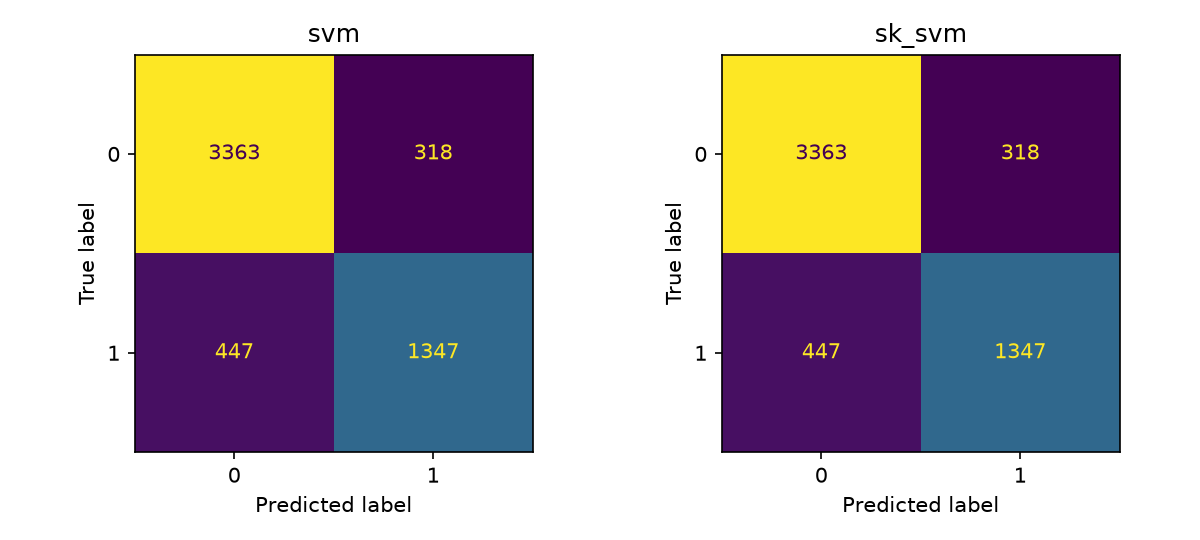
\includegraphics[width=0.85\textwidth]{confusion_svm}
	\caption{\textit{Confusion matrix} SVM \textit{from scratch} (kiri) dan \texttt{SVC} (kanan) pada \texttt{X\_val}}
	\label{fig:cm-svm}
\end{figure}

\begin{table}[H]
	\centering
	\caption{\textit{Classification report} SVM pada \texttt{X\_val} (sama untuk \textit{from scratch} dan \texttt{SVC})}
	\label{tab:report-svm}
	\begin{tabular}{l c c c r}
		\toprule
		\textbf{Kelas} & \textbf{\textit{Precision}} & \textbf{\textit{Recall}} & \textbf{F1} & \textbf{\textit{Support}} \\
		\midrule
		0 (tidak batal) & 0,8827 & 0,9136 & 0,8979 & 3.681 \\
		1 (batal)       & 0,8090 & 0,7508 & 0,7788 & 1.794 \\
		\midrule
		\textit{Accuracy}     & \multicolumn{3}{c}{0,8603} & 5.475 \\
		\textit{Macro avg}    & 0,8458 & 0,8322 & 0,8384 & 5.475 \\
		\bottomrule
	\end{tabular}
\end{table}

\subsection{Analisis}

Dari 1.794 pembatalan pada \texttt{X\_val}, SVM mendeteksi 1.347 pembatalan
(\textit{recall} 75\%) dan melewatkan 447 pembatalan (\textit{false negative}).
Sebanyak 318 pemesanan yang tidak batal salah diprediksi batal (\textit{false
positive}). F1 kelas batal (0,78) lebih rendah daripada F1 kelas tidak batal
(0,90). Kelas batal juga merupakan kelas yang jumlah sampelnya lebih sedikit.

Simpangan baku antar-\textit{fold} kecil (0,006), dan skor \textit{hold-out} dekat
dengan rata-rata \textit{k-fold}. Kinerja SVM tidak bergantung pada satu cara
pembagian data tertentu.

SVM RBF mengungguli Logistic Regression scikit-learn (0,8384 dan 0,7713). Selisih
ini mengindikasikan bahwa batas keputusan antara kedua kelas tidak linear sehingga
model linear dengan fitur yang sama tidak dapat menangkapnya sepenuhnya.

\texttt{GaussianNB} hanya mencapai 0,3773. Model ini mengasumsikan setiap fitur
berdistribusi normal dan saling bebas jika kelasnya diketahui. Banyak fitur pada
data ini berupa kolom \textit{one-hot} atau fitur diskret yang hampir konstan.
Kemungkinan penyebabnya adalah variansi yang sangat kecil pada fitur-fitur
tersebut sehingga \textit{likelihood}-nya mendominasi posterior. Dugaan ini belum
diuji.

\subsection{Seleksi Fitur SVM}

SVM linear ($C=0{,}1$) yang dilatih dengan tiga puluh fitur menghasilkan sepuluh
fitur dengan $|w|$ terbesar. Urutannya dari yang terbesar adalah
\texttt{special\_requests}, \texttt{days\_before\_arrival}, \texttt{date\_rate},
\texttt{lead\_x\_price}, \texttt{booking\_channel\_Online Travel Agent},
\texttt{booking\_channel\_Offline Agent}, \texttt{booking\_channel\_Complimentary},
\texttt{needs\_parking}, \texttt{is\_returning\_guest}, dan \texttt{doy\_cos}.
Dua fitur teratas sama dengan dua fitur yang nilai mutlak korelasinya terhadap
target paling besar pada Bab~1. Dua fitur hasil rekayasa, yaitu \texttt{date\_rate} dan
\texttt{lead\_x\_price}, berada di peringkat ketiga dan keempat.

Untuk melihat apakah seleksi fitur dan reduksi dimensi membantu, SVM RBF ($C=3$,
$\gamma=0{,}1$) dilatih dengan empat variasi masukan (Tabel~\ref{tab:seleksi}).
SVM RBF tidak memiliki bobot $w$ sehingga \texttt{Pipeline(select=k)} tidak dapat
meranking fiturnya sendiri. Karena itu, pada varian top-$k$, peringkat fitur
diambil dari $|w|$ SVM linear ($C=0{,}1$), lalu SVM RBF dilatih dengan $k$ fitur
teratas. Peringkat ini dihitung ulang pada setiap \textit{fold} agar data validasi
tidak ikut menentukan fitur yang dipilih. Varian PCA memakai
\texttt{Pipeline(pca=0.95)}, yang memilih 21 komponen untuk menjelaskan 95\%
variansi. Sebagai pembanding, SVM linear juga dievaluasi dengan tiga puluh fitur
dan dengan \texttt{Pipeline(select=10)}.

\begin{table}[H]
	\centering
	\caption{Pengaruh seleksi fitur dan PCA pada SVM}
	\label{tab:seleksi}
	\begin{tabular}{l l c c c}
		\toprule
		\textbf{Model} & \textbf{Masukan} & \textbf{\textit{Hold-out}} & \textbf{5-\textit{fold} $\mu$} & \textbf{5-\textit{fold} $\sigma$} \\
		\midrule
		SVM RBF    & 30 fitur                   & \textbf{0,8384} & \textbf{0,8328} & 0,0062 \\
		SVM RBF    & PCA (21 komponen)          & 0,8376 & 0,8305 & 0,0062 \\
		SVM RBF    & 20 fitur teratas           & 0,8219 & 0,8214 & 0,0042 \\
		SVM RBF    & 10 fitur teratas           & 0,7964 & 0,8013 & 0,0083 \\
		\midrule
		SVM linear & 30 fitur                   & 0,7705 & 0,7667 & 0,0077 \\
		SVM linear & 10 fitur teratas           & 0,7676 & 0,7651 & 0,0081 \\
		\bottomrule
	\end{tabular}
\end{table}

Seleksi fitur tidak membantu SVM RBF. Dengan dua puluh fitur teratas, rata-rata
5-\textit{fold} turun 0,0114, dan dengan sepuluh fitur teratas turun 0,0315.
Kemungkinan penyebabnya, peringkat dari SVM linear hanya mengukur kontribusi
linear setiap fitur, sedangkan fitur yang bobot linearnya kecil masih dapat
berguna bagi kernel RBF melalui interaksinya dengan fitur lain. Pada SVM
linear, seleksi sepuluh fitur hampir tidak mengubah skor (0,7651 dan 0,7667)
karena peringkatnya berasal dari model yang sama.

PCA dengan 21 komponen menghasilkan skor yang hampir sama dengan tiga puluh fitur
asli. Selisih rata-ratanya (0,0023) lebih kecil daripada simpangan baku
antar-\textit{fold} (0,0062). PCA mengurangi dimensi masukan sepertiga tanpa
penurunan skor yang berarti, tetapi juga tidak menaikkan skor. Karena itu, model
akhir tetap memakai tiga puluh fitur tanpa seleksi dan tanpa PCA.

\section{Hasil Bayesian Network}
\label{sec:hasil-bn}

\subsection{TAN Dibandingkan \textit{Naive Bayes}}

\textit{Naive Bayes} dan TAN memakai diskretisasi, CPT, dan 5 \textit{bin} yang
sama. Satu-satunya perbedaan adalah struktur: TAN menambahkan satu
\textit{parent} fitur per fitur (Subbab~\ref{sec:tan}). Pada Tabel~\ref{tab:perbandingan},
TAN mencapai \textit{macro F1} 5-\textit{fold} 0,7624 ($\sigma=0{,}0066$)
berbanding 0,7119 ($\sigma=0{,}0049$) untuk \textit{Naive Bayes}. Selisih 0,0505
jauh lebih besar daripada simpangan baku antar-\textit{fold}. Pada \textit{hold-out},
selisihnya 0,0634 (0,7617 berbanding 0,6983). Besarnya berbeda dari 5-\textit{fold},
tetapi arahnya sama pada kedua cara evaluasi.

Diskretisasi juga memperbaiki \textit{Naive Bayes} secara besar dibandingkan
\texttt{GaussianNB} (0,7119 berbanding 0,3804) dengan asumsi kebebasan yang sama.
Hasil ini sejalan dengan dugaan pada bab sebelumnya bahwa distribusi normal tidak
cocok untuk fitur \textit{one-hot} dan fitur diskret pada data ini. Dugaan
tersebut belum diuji secara langsung.

\begin{table}[H]
	\centering
	\caption{\textit{Classification report} \textit{Naive Bayes}, TAN, dan KDB ($k=10$) pada \texttt{X\_val}}
	\label{tab:report-bn}
	\begin{tabular}{l l c c c}
		\toprule
		\textbf{Model} & \textbf{Kelas} & \textbf{\textit{Precision}} & \textbf{\textit{Recall}} & \textbf{F1} \\
		\midrule
		\textit{Naive Bayes} & 0 (tidak batal) & 0,8246 & 0,7446 & 0,7826 \\
		                     & 1 (batal)       & 0,5630 & 0,6750 & 0,6139 \\
		\midrule
		TAN                  & 0 (tidak batal) & 0,8374 & 0,8587 & 0,8479 \\
		                     & 1 (batal)       & 0,6941 & 0,6577 & 0,6754 \\
		\midrule
		KDB ($k=10$)         & 0 (tidak batal) & 0,8550 & 0,9242 & 0,8883 \\
		                     & 1 (batal)       & 0,8135 & 0,6784 & 0,7398 \\
		\bottomrule
	\end{tabular}
\end{table}

\textit{Naive Bayes} memprediksi 39,3\% baris \texttt{X\_val} sebagai batal,
padahal proporsi pembatalan sebenarnya 32,8\%. Kelebihan prediksi batal ini
terlihat pada \textit{precision} kelas batal yang rendah (0,5630) dan 940
\textit{false positive}. TAN memprediksi 31,1\% baris sebagai batal, hampir sama
dengan proporsi sebenarnya, dengan \textit{false positive} turun menjadi 520.
Penyebab yang mungkin adalah informasi ganda dari fitur yang saling berkaitan
pada \textit{Naive Bayes}. Penyebab ini sejalan dengan struktur TAN pada
Subbab berikutnya, tetapi belum diuji dengan menghapus fitur yang berkaitan.

\subsection{Struktur yang Dipelajari TAN}

Dari 666 pasangan fitur yang mungkin, TAN memilih 36 edge. Edge dengan
\textit{conditional mutual information} terbesar adalah pasangan fitur yang
diturunkan dari fitur yang sama: \texttt{arrival\_month} $\to$ \texttt{month\_cos}
(1,150), \texttt{month\_sin} $\to$ \texttt{doy\_sin} (1,113),
\texttt{arrival\_month} $\to$ \texttt{month\_sin} (1,093), dan
\texttt{month\_cos} $\to$ \texttt{doy\_cos} (0,867). Pasangan berikutnya juga
bersifat turunan: \texttt{num\_adults} $\to$ \texttt{total\_guests} (0,609),
\texttt{weekday\_nights} $\to$ \texttt{total\_nights} (0,494), dan
\texttt{lead\_x\_price} $\to$ \texttt{days\_before\_arrival} (0,333). Ada pula
pasangan dua kolom \textit{one-hot} dari satu atribut, yaitu
\texttt{booking\_channel\_Online Travel Agent} $\to$
\texttt{booking\_channel\_Offline Agent} (0,432): jika satu kolom bernilai 1,
kolom lain pasti 0. Ini adalah pasangan yang menyebabkan \textit{Naive Bayes}
menghitung informasi yang sama berulang kali. Nilai terkecil di antara edge
terpilih kurang dari 0,001, yaitu hubungan yang hampir tidak ada
(Gambar~\ref{fig:graf-bn}).

Harga dari struktur ini adalah ukuran tabel. Jumlah sel CPT (seluruh nilai
probabilitas yang disimpan) naik dari 240 pada \textit{Naive Bayes} menjadi 918
pada TAN. CPT terbesar berukuran
$2\times5\times5=50$ sel (misalnya pada \texttt{days\_before\_arrival}).
Tabel yang lebih besar membutuhkan data lebih banyak, tetapi dengan 21.898 baris
latih ini belum menimbulkan masalah yang terlihat.

\subsection{KDB: Lebih dari Satu \textit{Parent}}
\label{sec:hasil-kdb}

KDB (Subbab~\ref{sec:kdb}) dievaluasi dengan diskretisasi dan 5 \textit{bin}
yang sama, sehingga satu-satunya perbedaan dengan TAN adalah jumlah
\textit{parent} fitur. Tabel~\ref{tab:kdb} menunjukkan pengaruh $k$.

\begin{table}[H]
	\centering
	\caption{Pengaruh $k$ pada KDB (\texttt{n\_bins}=5, \textit{macro F1})}
	\label{tab:kdb}
	\begin{tabular}{c c c c r}
		\toprule
		$k$ & \textbf{\textit{Hold-out}} & \textbf{5-\textit{fold} $\mu$} & \textbf{5-\textit{fold} $\sigma$} & \textbf{Sel CPT padat} \\
		\midrule
		0 (\textit{Naive Bayes}) & 0,6983 & 0,7119 & 0,0049 & 240 \\
		1 & 0,7630 & 0,7695 & 0,0041 & 968 \\
		2 & 0,7718 & 0,7744 & 0,0080 & 4.312 \\
		3 & 0,7826 & 0,7836 & 0,0045 & 18.476 \\
		4 & 0,7827 & 0,7925 & 0,0051 & 60.840 \\
		5 & 0,7893 & 0,7956 & 0,0019 & 221.990 \\
		6 & 0,8023 & 0,8009 & 0,0078 & 911.060 \\
		8 & 0,8069 & 0,8032 & 0,0022 & $1{,}3\times10^{7}$ \\
		\textbf{10} & \textbf{0,8140} & \textbf{0,8117} & 0,0072 & $1{,}7\times10^{8}$ \\
		12 & 0,8125 & 0,8101 & 0,0051 & $1{,}7\times10^{9}$ \\
		16 & 0,8041 & 0,8006 & 0,0043 & $2{,}7\times10^{11}$ \\
		29 & 0,7930 & 0,7937 & 0,0056 & $3{,}1\times10^{16}$ \\
		\bottomrule
	\end{tabular}
\end{table}

Skor naik seiring $k$ sampai sekitar $k=10$, lalu turun. Dari TAN (0,7624) ke KDB
$k=10$ (0,8117), \textit{macro F1} 5-\textit{fold} naik 0,0493, tujuh kali
simpangan bakunya. KDB $k=1$ (0,7695) sedikit di atas TAN walaupun keduanya
memberi satu \textit{parent} per fitur. Bedanya, KDB memilih \textit{parent}
berdasarkan urutan $I(X_i;C)$, sedangkan TAN memilih pohon dengan total bobot
terbesar.

Penurunan setelah $k=10$ sejalan dengan jumlah data. Dengan 21.898 baris latih,
makin banyak \textit{parent}, makin sedikit baris yang jatuh pada setiap
kombinasi nilai \textit{parent}. Sel CPT padat pada $k=10$ sudah
$1{,}7\times10^{8}$, sedangkan hitungan yang benar-benar tersimpan sebagai CPT
\textit{sparse} hanya sekitar 430 ribu. Sebagian besar peluang akhirnya hanya
berasal dari \textit{smoothing}. Nilai di sekitarnya hampir setara: $k=9$
mendapat 0,8059, $k=11$ mendapat 0,8125, dan $k=12$ mendapat 0,8101. Selisih
terbesarnya 0,0066, sebanding dengan simpangan baku, sehingga rentang $k=9$
sampai 12 tidak dapat dibedakan secara meyakinkan.

Nilai $k=10$ dipilih sebagai model akhir karena berada di rentang tersebut dengan
CPT lebih kecil daripada $k=11$ dan $k=12$. Pada $k=10$, \texttt{alpha} 0,5 dan 2
memberi 0,8085 dan 0,8120, sehingga \texttt{alpha}=1 dipertahankan. Nilai
\texttt{n\_bins} 4 dan 6 memberi 0,8119 dan 0,8070. Empat \textit{bin} setara
dengan lima, sehingga 5 \textit{bin} dipertahankan agar sama dengan
\textit{Naive Bayes} dan TAN.

Pada \texttt{X\_val}, KDB $k=10$ mencapai akurasi 0,8437 dan memprediksi 27,3\%
baris sebagai batal. \textit{Precision} kelas batal naik menjadi 0,8135
(TAN 0,6941) dan \textit{recall}-nya juga naik menjadi 0,6784 (TAN 0,6577).
\textit{False positive} turun dari 520 pada TAN menjadi 279.

\todo{Isi skor Kaggle KDB $k=10$ dari \texttt{output/bn\_kdb10.csv} setelah
berkas itu diunggah, lalu bandingkan dengan \textit{macro F1} \textit{hold-out}
(0,8140).}

\subsection{Pengaruh \texttt{n\_bins}}
\label{sec:tuning-bn}

Jumlah \textit{bin} dipilih dengan \textit{grid search} 5-\textit{fold}
(Tabel~\ref{tab:tuning-bn}).

\begin{table}[H]
	\centering
	\caption{Hasil \textit{tuning} \texttt{n\_bins} pada Bayesian Network}
	\label{tab:tuning-bn}
	\begin{tabular}{c c c c c}
		\toprule
		& \multicolumn{2}{c}{\textbf{\textit{Naive Bayes}}} & \multicolumn{2}{c}{\textbf{TAN}} \\
		\cmidrule(lr){2-3}\cmidrule(lr){4-5}
		\textbf{\texttt{n\_bins}} & \textbf{5-\textit{fold} $\mu$} & \textbf{5-\textit{fold} $\sigma$} & \textbf{5-\textit{fold} $\mu$} & \textbf{5-\textit{fold} $\sigma$} \\
		\midrule
		3  & \textbf{0,7148} & 0,0070 & 0,7460 & 0,0056 \\
		5  & 0,7119 & 0,0049 & \textbf{0,7624} & 0,0066 \\
		10 & 0,7116 & 0,0042 & 0,7570 & 0,0056 \\
		\bottomrule
	\end{tabular}
\end{table}

Pada \textit{Naive Bayes}, ketiga nilai \texttt{n\_bins} praktis setara karena
selisih terbesar (0,0032) lebih kecil daripada simpangan baku (0,004--0,007).
Pada TAN, \texttt{n\_bins}=5 terbaik, sedangkan 3 \textit{bin} turun 0,0164 dan 10
\textit{bin} turun 0,0054. Penurunan pada 10 \textit{bin} masih sebanding dengan
simpangan baku, sehingga hanya 3 \textit{bin} yang jelas lebih buruk.
Kemungkinan penyebabnya, 3 \textit{bin} terlalu kasar untuk menangkap hubungan
antarfitur. Dugaan ini belum diuji.

\subsection{Klasifikasi Sensitif-Biaya}

Aturan keputusan dengan $C_{FP}=2$ dan $C_{FN}=1$ (Subbab~\ref{sec:biaya-bn}) dievaluasi pada
\texttt{X\_val} dengan biaya total $2\cdot FP+FN$ (Tabel~\ref{tab:biaya-bn}).

\begin{table}[H]
	\centering
	\caption{Pengaruh aturan keputusan sensitif-biaya pada \texttt{X\_val} (Batal = persentase baris yang diprediksi batal)}
	\label{tab:biaya-bn}
	\small
	\begin{tabular}{l r r r c c}
		\toprule
		\textbf{Model} & \textbf{FP} & \textbf{FN} & \textbf{Biaya $2\,FP+FN$} & \textbf{\textit{Macro F1}} & \textbf{Batal (\%)} \\
		\midrule
		\textit{Naive Bayes}              & 940 & 583 & 2.463 & 0,6983 & 39,3 \\
		\textit{Naive Bayes} + biaya      & 704 & 689 & 2.097 & 0,7119 & 33,0 \\
		TAN                               & 520 & 614 & 1.654 & 0,7617 & 31,1 \\
		TAN + biaya                       & 285 & 845 & 1.415 & 0,7421 & 22,5 \\
		KDB ($k=10$)                      & 279 & 577 & 1.135 & 0,8140 & 27,3 \\
		KDB ($k=10$) + biaya              & 222 & 626 & 1.070 & 0,8122 & 25,4 \\
		\bottomrule
	\end{tabular}
\end{table}

Aturan sensitif-biaya menurunkan biaya total pada ketiga model: dari 2.463 ke 2.097
(turun 14,9\%) pada \textit{Naive Bayes}, dari 1.654 ke 1.415 (turun 14,5\%)
pada TAN, dan dari 1.135 ke 1.070 (turun 5,7\%) pada KDB. Penurunan pada KDB
paling kecil karena KDB sudah lebih jarang memprediksi batal (279
\textit{false positive}). \textit{False positive} turun dan \textit{false negative}
naik, sesuai dengan harga yang diasumsikan. \textit{Macro F1} tidak otomatis ikut
naik: pada TAN justru turun (0,7617 menjadi 0,7421) karena \textit{macro F1}
menganggap semua kesalahan sama berat, sedangkan yang dioptimalkan adalah biaya.
Pada \textit{Naive Bayes} \textit{macro F1} naik (0,6983 menjadi 0,7119) karena
model ini semula terlalu sering memprediksi batal. Pemilihan antara
\textit{macro F1} dan biaya bergantung pada metrik yang dianggap utama. Metrik
penilaian tugas ini adalah \textit{macro F1}, sehingga aturan sensitif-biaya
dilaporkan sebagai bonus dan tidak dipakai pada perbandingan utama
(Tabel~\ref{tab:perbandingan}).

\section{\textit{Hyperparameter Tuning}}

\textit{Tuning} dijalankan dengan fungsi \texttt{tune}, yaitu \textit{grid search}
yang menilai setiap kombinasi parameter dengan rata-rata \textit{macro F1}
5-\textit{fold} pada \texttt{X\_train}. Untuk SVM, \textit{grid} pada
\textit{notebook} memvariasikan $C\in\{1,3,5\}$ dengan kernel RBF dan
$\gamma=0{,}1$ tetap (Tabel~\ref{tab:tuning-svm}). Kelima belas pelatihan
(tiga kombinasi $\times$ lima \textit{fold}) selesai dalam 172 detik.

\begin{table}[H]
	\centering
	\caption{Hasil \textit{tuning} SVM RBF ($\gamma=0{,}1$)}
	\label{tab:tuning-svm}
	\begin{tabular}{c c c}
		\toprule
		$C$ & \textbf{5-\textit{fold} $\mu$} & \textbf{5-\textit{fold} $\sigma$} \\
		\midrule
		1 & 0,8288 & 0,0034 \\
		3 & \textbf{0,8328} & 0,0062 \\
		5 & 0,8322 & 0,0064 \\
		\bottomrule
	\end{tabular}
\end{table}

Nilai $C=3$ memberikan rata-rata tertinggi (0,8328) dan dipilih sebagai
konfigurasi akhir. Menaikkan $C$ dari 1 ke 3 menambah 0,0040, sedangkan menaikkan
$C$ dari 3 ke 5 justru menurunkan skor sebesar 0,0006. Selisih antara $C=3$ dan
$C=5$ jauh lebih kecil daripada simpangan baku antar-\textit{fold} (sekitar
0,006) sehingga keduanya praktis setara. Semakin besar $C$, semakin besar pula
hukuman untuk sampel yang melanggar margin. Pada rentang ini, kenaikan $C$ di atas
3 tidak lagi memperbaiki skor validasi.

Model akhir ($C=3$) yang dilatih pada \texttt{X\_train} konvergen setelah 30.419
iterasi SMO dan memiliki 9.039 \textit{support vector} (41\% dari 21.857 baris).
Sebanyak 5.131 di antaranya memiliki $\alpha=C$, yaitu sampel yang berada di
dalam margin atau salah diklasifikasikan pada data latih. Jumlah ini mengindikasikan
bahwa kedua kelas banyak beririsan pada ruang fitur.

\todo{Tambahkan hasil \textit{tuning} KNN ($k\in\{5,15,31\}$), Logistic Regression
($\texttt{lr}\in\{0{,}01;0{,}1\}$), dan DTL ($\texttt{max\_depth}\in\{5,8,\text{None}\}$)
serta tabel \texttt{ranking} semua model. \textit{Tuning} Bayesian Network ada pada
Subbab~\ref{sec:tuning-bn}.}

\section{Analisis Kesalahan}

SVM hasil \textit{tuning} salah memprediksi 765 dari 5.475 baris \texttt{X\_val}
(14,0\%), terdiri atas 447 \textit{false negative} dan 318 \textit{false
positive} (Gambar~\ref{fig:cm-svm}). Jumlah \textit{false negative} yang lebih
besar sesuai dengan proporsi prediksi batal: model memprediksi 30,4\% baris
\texttt{X\_val} sebagai batal, sedangkan proporsi pembatalan sebenarnya 32,8\%.

Untuk mencari pola kesalahan, baris \texttt{X\_val} dikelompokkan menjadi
\textit{true positive} (TP), \textit{true negative} (TN), \textit{false positive}
(FP), dan \textit{false negative} (FN), lalu nilai fitur aslinya dibandingkan.
Median \textit{lead time} kelompok TP adalah 161 hari dan kelompok TN 37 hari.
Kesalahan berada di antara keduanya: median FN 62 hari dan median FP 80 hari.
Pola yang sama terlihat pada permintaan khusus. Proporsi pemesanan tanpa
permintaan khusus adalah 68,6\% pada TP dan 37,8\% pada TN, sedangkan pada FP
61,3\% dan pada FN 42,3\%. Dengan kata lain, pembatalan yang terlewat (FN) memiliki
ciri yang mirip dengan pemesanan yang tidak batal, dan pemesanan yang salah
diprediksi batal (FP) memiliki ciri yang mirip dengan pembatalan.

\begin{table}[H]
	\centering
	\caption{Tingkat kesalahan SVM pada \texttt{X\_val} berdasarkan \textit{lead time}}
	\label{tab:error-lead}
	\begin{tabular}{l r c c r r}
		\toprule
		\textbf{\textit{Lead time} (hari)} & \textbf{Baris} & \textbf{Rasio batal} & \textbf{Tingkat kesalahan} & \textbf{FN} & \textbf{FP} \\
		\midrule
		0-7     & 802   & 0,086 & 0,072 & 42  & 16 \\
		8-30    & 965   & 0,181 & 0,123 & 71  & 48 \\
		31-90   & 1.562 & 0,256 & 0,159 & 149 & 99 \\
		91-180  & 1.133 & 0,457 & 0,211 & 122 & 117 \\
		$>180$   & 767   & 0,722 & 0,065 & 24  & 26 \\
		\bottomrule
	\end{tabular}
\end{table}

Tabel~\ref{tab:error-lead} menunjukkan bahwa tingkat kesalahan tertinggi
(21,1\%) terjadi pada \textit{lead time} 91-180 hari, yaitu rentang dengan rasio
pembatalan paling dekat dengan 50\%. Pada \textit{lead time} sangat pendek
($\le 7$ hari) dan sangat panjang ($>180$ hari), sebagian besar pemesanan berada
di satu kelas sehingga tingkat kesalahannya di bawah 8\%. Sebanyak 246 baris
dengan \textit{lead time} kosong pada data mentah tidak masuk ke tabel ini.

Tingkat kesalahan juga berbeda antarkanal pemesanan. Tingkat kesalahan pada Online
Travel Agent adalah 17,9\% (3.519 baris), sedangkan pada Offline Agent 6,9\%
(1.573 baris) dan pada Corporate 8,1\% (309 baris). Rasio pembatalan Online Travel
Agent (36,2\%) dan Offline Agent (30,8\%) tidak jauh berbeda, tetapi pembatalan
pada Online Travel Agent lebih sulit dipisahkan oleh fitur yang tersedia. Fitur
tambahan yang membedakan pemesanan pada kanal ini dapat menjadi arah perbaikan.

\todo{Tambahkan \textit{confusion matrix} model lain setelah \textit{tuning}.}

\section{Prediksi Data Uji}

Model akhir, yaitu SVM RBF dengan $C=3$ dan $\gamma=0{,}1$, dilatih ulang dengan
gabungan \texttt{X\_train} dan \texttt{X\_val} (27.332 baris). Pelatihan ini
konvergen setelah 37.842 iterasi SMO dengan 10.927 \textit{support vector}.
Prediksi untuk 6.844 baris \texttt{X\_test} disimpan di
\texttt{output/svm\_20261121-120000.csv}, dan modelnya disimpan di berkas
\texttt{.pkl} dengan nama yang sama. Model memprediksi 29,8\% baris data uji
sebagai batal, mendekati proporsi prediksi batal pada \texttt{X\_val} (30,4\%).

Prediksi pada berkas ini identik dengan prediksi pada submisi Kaggle sebelumnya
(\texttt{svm\_20261120-214807.csv}) untuk seluruh 6.844 baris. Submisi tersebut
memperoleh skor 0,84979 pada Kaggle. Skor tersebut lebih
tinggi daripada \textit{macro F1} \textit{hold-out} (0,8384) dan rata-rata
5-\textit{fold} (0,8328). Salah satu kemungkinan penyebabnya adalah jumlah data
latih model akhir yang 25\% lebih banyak, tetapi selisih ini juga dapat berasal
dari perbedaan sampel data uji.
